\section*{WU4}
\begin{figure}[here]
	\center
	\caption{wu4: Plot of circular data that are generated with shared center.}
	\label{fig:wu4}
	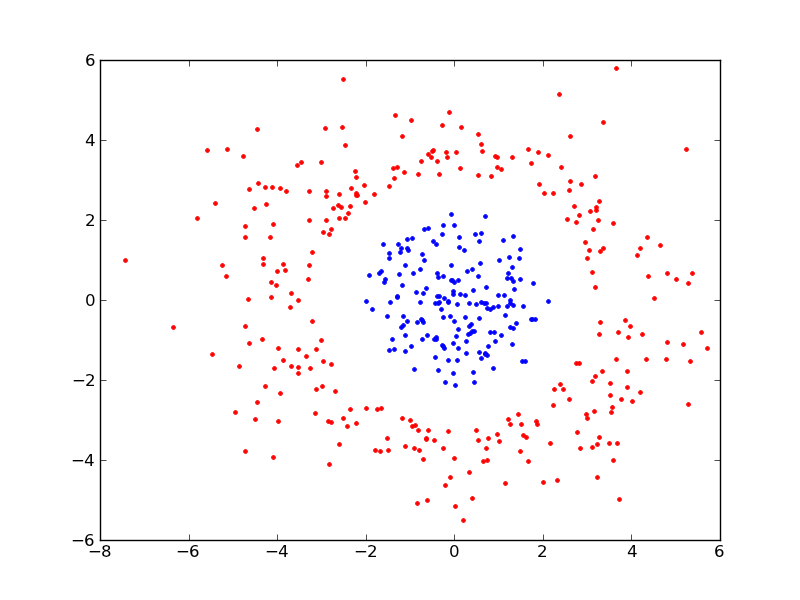
\includegraphics[width=4.0in]{img/wu4.png}
\end{figure}
Figure \ref{fig:wu4} shows the plot of the data. 
Vanilla PCA will find this data difficult because the variance in all directions is similar. This means that eigenvectors can point in any direction.

The large eigenvalues have no significance. For example, with a poly3 kernel, the eigenvalues are ridiculously 
large due to cubing the dot product. What does hold significance, however, is the normalized eigenvalues. 

\section*{WU5}
\begin{figure}[here]
	\center
	\caption{wu5: Plot of data points transformed by vanilla PCA}
	\label{fig:wu5}
	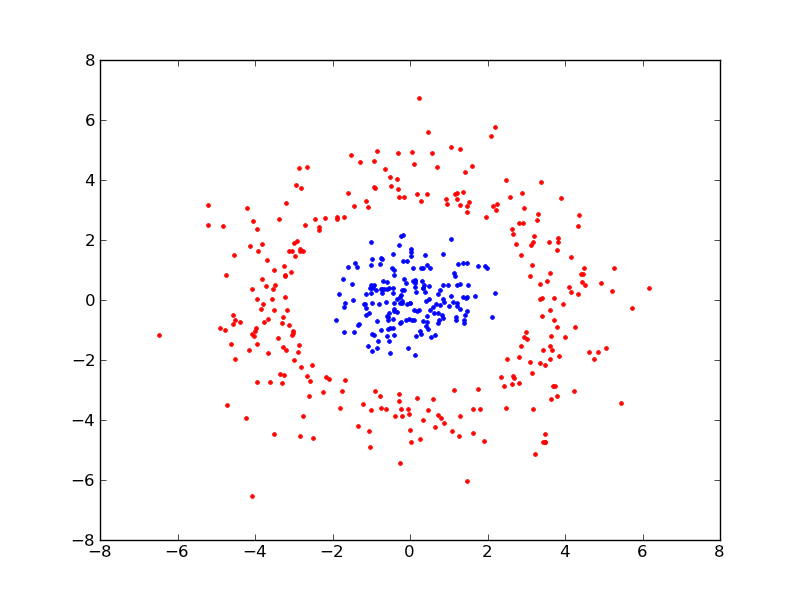
\includegraphics[width=4.0in]{img/wu5.png}
\end{figure}

Figure \ref{fig:wu5} shows the result of PCA. 
PCA did not do what we want it to do :'(
In addition to the reasons listed in WU4, vanilla PCA 
did not do what we wanted to do because the resulting data 
is not linearly separable.

\section*{WU6}
\begin{figure}[here]
	\center
	\caption{wu6}
	\label{fig:wu6}
	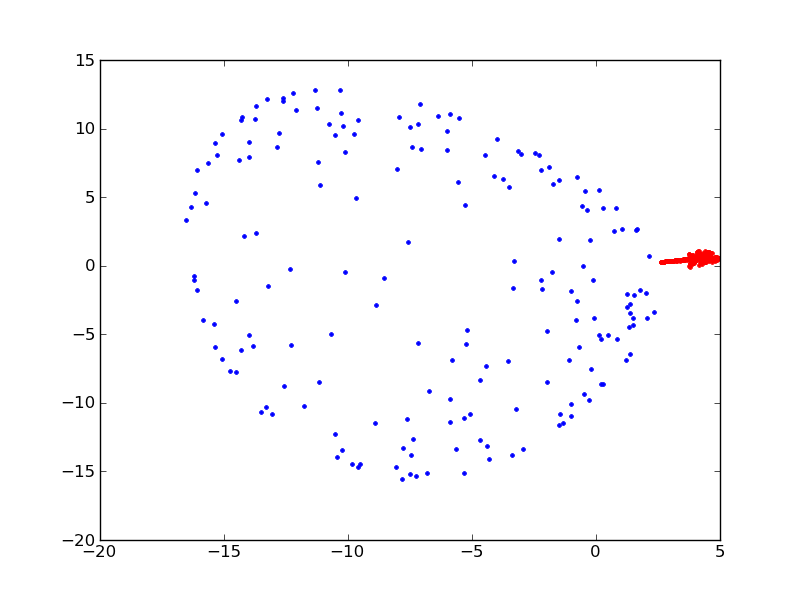
\includegraphics[width=4.0in]{img/wu7_rbf1.png}
\end{figure}

The eigenvalues for KPCA with rbf1 kernel is [ 0.08270371  0.07927822], which is significantly smaller than
the eigenvalues for KPCA with linear kernel: [ 5.68035099  1.51738947]. This means that the rbf1 kernel does a much 
better job at making the data linearly separable than the linear kernel. See the Figure \ref{fig:wu7_rbf1} for a plot of the rbf1 kernel and Figure \ref{fig:wu7_linear} for the plot of the linear kernel for a visual comparison.

\section*{WU7}
\begin{verbatim}
	linear: [ 6.1633096   5.75720649]
	poly2: [ 64.10397019  62.76778803]
	poly3: [ 2906.46175423  2477.34358423]
	rbf0_2: [ 0.14538657  0.10079059]
	rbf0_5: [ 0.11223664  0.06506837]
	rbf1: [ 0.07796779  0.05559504]
	rbf2: [ 0.05140468  0.04200365]
	rbf5: [ 0.02830142  0.02551005]

\end{verbatim}
Plots for the various kernels:
\begin{itemize}
	\item linear: Figure \ref{fig:wu7_linear}
	\item poly2: Figure \ref{fig:wu7_poly2}
	\item poly3: Figure \ref{fig:wu7_poly3}
	\item rbf0.2: Figure \ref{fig:wu7_rbf0_2}
	\item rbf0.5: Figure \ref{fig:wu7_rbf0_5}
	\item rbf2: Figure \ref{fig:wu7_rbf2}
	\item rbf5: Figure \ref{fig:wu7_rbf5}
\end{itemize}


\begin{figure}[here]
	\center
	\caption{wu7: KPCA with a linear kernel}
	\label{fig:wu7_linear}
	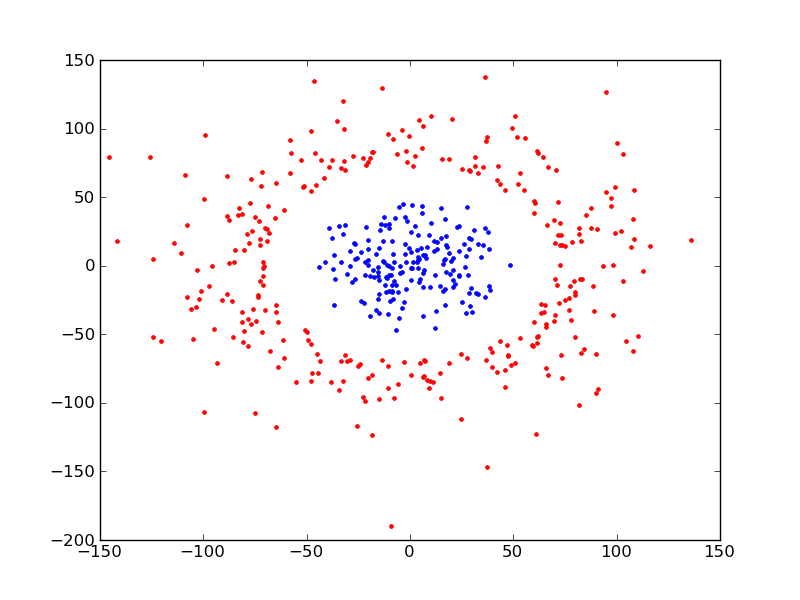
\includegraphics[width=4.0in]{img/wu7_linear.png}
\end{figure}

\begin{figure}[here]
	\center
	\caption{wu7: KPCA with a poly2 kernel}
	\label{fig:wu7_poly2}
	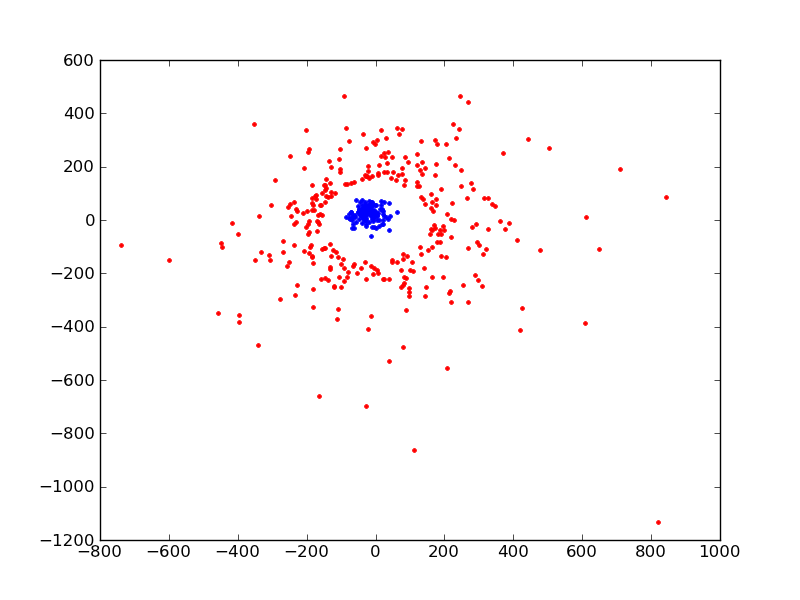
\includegraphics[width=4.0in]{img/wu7_poly2.png}
\end{figure}

\begin{figure}[here]
	\center
	\caption{wu7: KPCA with a poly3 kernel}
	\label{fig:wu7_poly3}
	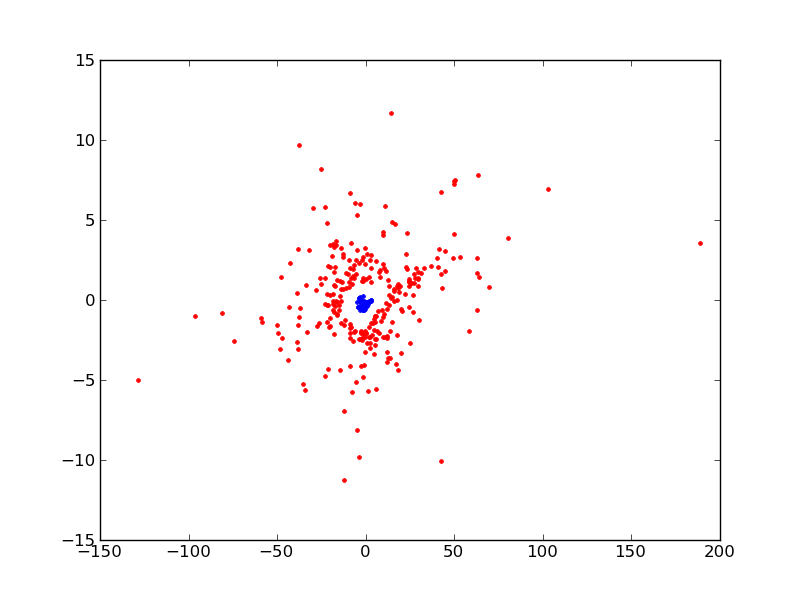
\includegraphics[width=4.0in]{img/wu7_poly3.png}
\end{figure}

\begin{figure}[here]
	\center
	\caption{wu7: KPCA with a rbf0.2 kernel}
	\label{fig:wu7_rbf0_2}
	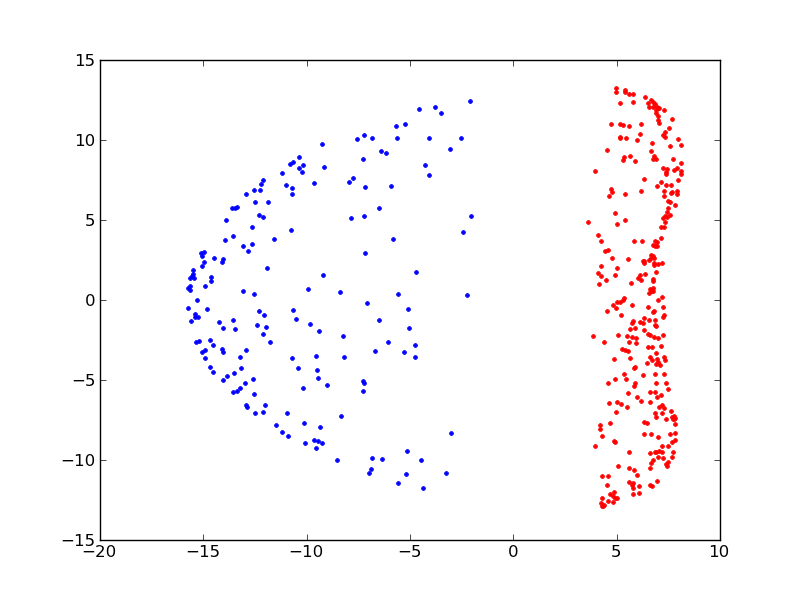
\includegraphics[width=4.0in]{img/wu7_rbf0_2.png}
\end{figure}

\begin{figure}[here]
	\center
	\caption{wu7: KPCA with a rbf0.5 kernel}
	\label{fig:wu7_rbf0_5}
	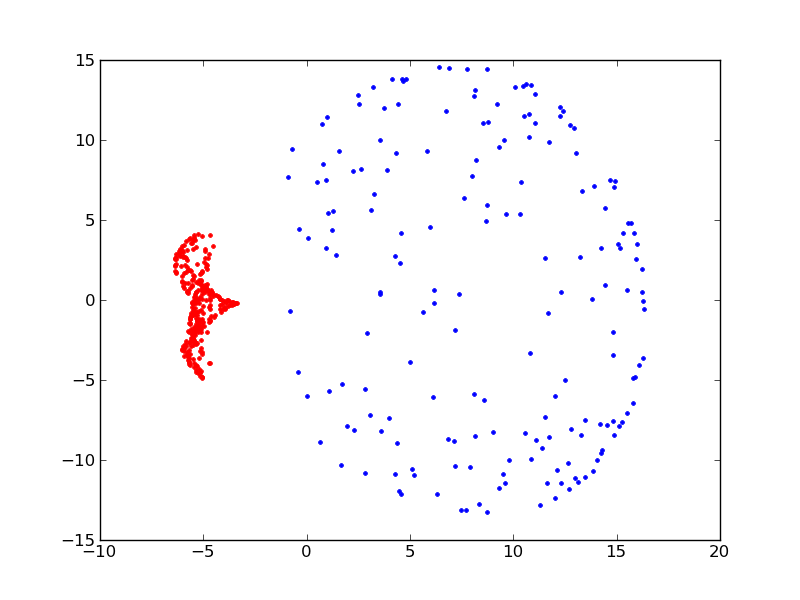
\includegraphics[width=4.0in]{img/wu7_rbf0_5.png}
\end{figure}

\begin{figure}[here]
	\center
	\caption{wu7: KPCA with a rbf1 kernel}
	\label{fig:wu7_rbf1}
	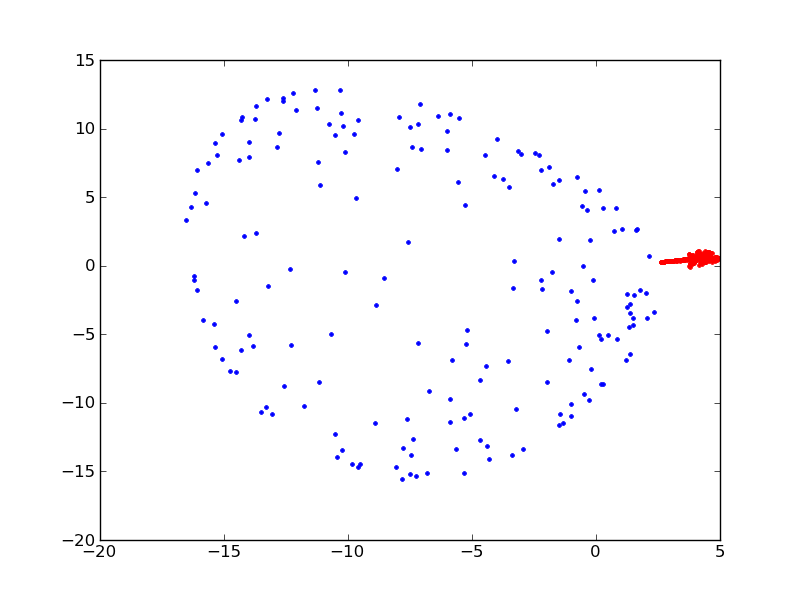
\includegraphics[width=4.0in]{img/wu7_rbf1.png}
\end{figure}

\begin{figure}[here]
	\center
	\caption{wu7: KPCA with a rbf2 kernel}
	\label{fig:wu7_rbf2}
	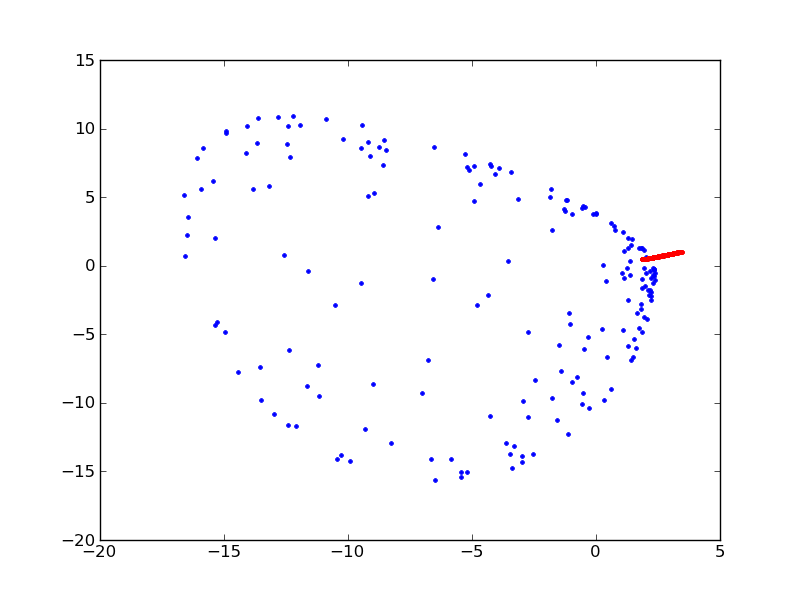
\includegraphics[width=4.0in]{img/wu7_rbf2.png}
\end{figure}

\begin{figure}[here]
	\center
	\caption{wu7: KPCA with a rbf5 kernel}
	\label{fig:wu7_rbf5}
	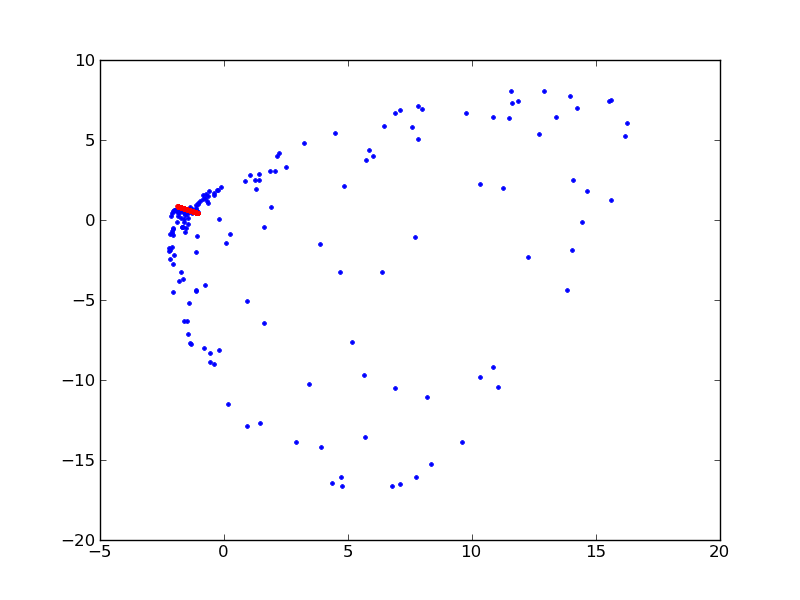
\includegraphics[width=4.0in]{img/wu7_rbf5.png}
\end{figure}